%%%%%%%%%%%%%%%%%%%%%%%%%%%%%%%%%%%%%%%%%%%%%%%%%%%%%%%%%%%%%%%%%%%%%%
% amspaper.tex --  LaTeX-based template for submissions to American 
% Meteorological Society journals
%
% Template developed by Amy Hendrickson, 2013, TeXnology Inc., 
% amyh@texnology.com, http://www.texnology.com
% following earlier work by Brian Papa, American Meteorological Society
%
% Email questions to latex@ametsoc.org.
%
%%%%%%%%%%%%%%%%%%%%%%%%%%%%%%%%%%%%%%%%%%%%%%%%%%%%%%%%%%%%%%%%%%%%%
% PREAMBLE
%%%%%%%%%%%%%%%%%%%%%%%%%%%%%%%%%%%%%%%%%%%%%%%%%%%%%%%%%%%%%%%%%%%%%

%% Start with one of the following:
% DOUBLE-SPACED VERSION FOR SUBMISSION TO THE AMS
\documentclass{ametsoc}

% TWO-COLUMN JOURNAL PAGE LAYOUT---FOR AUTHOR USE ONLY
% \documentclass[twocol]{ametsoc}

%%%%%%%%%%%%%%%%%%%%%%%%%%%%%%%%
%%% To be entered only if twocol option is used

\journal{jamc}

%  Please choose a journal abbreviation to use above from the following list:
% 
%   jamc     (Journal of Applied Meteorology and Climatology)
%   jtech     (Journal of Atmospheric and Oceanic Technology)
%   jhm      (Journal of Hydrometeorology)
%   jpo     (Journal of Physical Oceanography)
%   jas      (Journal of Atmospheric Sciences)	
%   jcli      (Journal of Climate)
%   mwr      (Monthly Weather Review)
%   wcas      (Weather, Climate, and Society)
%   waf       (Weather and Forecasting)
%   bams (Bulletin of the American Meteorological Society)
%   ei    (Earth Interactions)

%%%%%%%%%%%%%%%%%%%%%%%%%%%%%%%%
%Citations should be of the form ``author year''  not ``author, year''
\bibpunct{(}{)}{;}{a}{}{,}

%%%%%%%%%%%%%%%%%%%%%%%%%%%%%%%%

%%% To be entered by author:

%% May use \\ to break lines in title:

\title{Assessment of the variability of the thermodynamic structure of the atmosphere in the Aburrá Valley, Colombia. Part I: Influence on precipitation}

%%% Enter authors' names, as you see in this example:
%%% Use \correspondingauthor{} and \thanks{Current Affiliation:...}
%%% immediately following the appropriate author.
%%%
%%% Note that the \correspondingauthor{} command is NECESSARY.
%%% The \thanks{} commands are OPTIONAL.

    \authors{Carlos Mario Cuervo López, Alejandra Isaza and CH\thanks{Universidad Nacional de Colombia, Medellín, Colombia.} \thanks{Sistema de Alerta Temprana de Medellín y el Valle de Aburrá (SIATA)}}

     \affiliation{Universidad Nacional de Colombia, Medellín, Colombia}

\email{cmcuervol@gmail.com}




%%%%%%%%%%%%%%%%%%%%%%%%%%%%%%%%%%%%%%%%%%%%%%%%%%%%%%%%%%%%%%%%%%%%%
% ABSTRACT
%
% Enter your Abstract here

\abstract{Precipitation is one of the most outstanding, dynamic and intermittent components of the hydrological cycle, therefore of the climatic system. Water vapour, being one of the factors conditioning precipitation, plays a crucial role in different atmospheric processes. Water vapour varies in a wide range of temporal and spatial scales, from the local scale associated with microclimatic variability, to global scales associated with long-term climate change. The distribution of water vapour is related to cloud distribution, precipitation and atmospheric storms due to the amount of latent heat released in the water’s phase change, which is also an important source of energy for air movement in the atmosphere. Besides, the distribution of water affects the vertical stability of the atmosphere, the structure and evolution of atmospheric storms, because these processes have great sensitivity to water vapour and temperature profiles, while also having implications in regional and global water and energy cycles. This research evaluates the variability of water vapour over the Aburrá Valley and its role on different thermodynamic processes of the troposphere at the start of precipitation events, mainly in events of convective origin. Different strategies were used, using remote and direct monitoring of the variables associated with thermodynamic processes in the atmosphere such as satellite sources like NASA’s AIRS (Atmospheric Infrared Sounder) products microwave radiometers (MWR ; \textit{MicroWave Radiometer}), 120 radiosoundings; finally applying modeling strategies to these processes using  the early warning system of Aburrá Valley (SIATA) operational numerical modeling scheme, which is based on the WRF (Weather Research Forecast) model. With these different strategies, water vapour and temperature profiles were obtained. The behaviour of the thermodynamic vertical structure of the atmosphere was quantified using stability indexes, which evaluates the effectiveness of nowcasting of precipitation events over the Aburrá Valley. It also shows some of the stability conditions and in general the thermodynamic conditions that favour the dispersion of pollutants. In these processes, the importance of having permanent measurements of the thermodynamic profiles of the troposphere was evidenced, mainly in the levels which are closer to the surface. where a better understanding of the thermodynamic phenomena associated with precipitation events and knowledge of the proper distribution of water vapour is needed not only during the beginning of the events but also during its extension and development with its drastic implications to air quality in the valley, mainly in terms of the extension of the atmospheric boundary layer.}



\begin{document}

%% Necessary!
\maketitle


%%%%%%%%%%%%%%%%%%%%%%%%%%%%%%%%%%%%%%%%%%%%%%%%%%%%%%%%%%%%%%%%%%%%%
% MAIN BODY OF PAPER
%%%%%%%%%%%%%%%%%%%%%%%%%%%%%%%%%%%%%%%%%%%%%%%%%%%%%%%%%%%%%%%%%%%%%
%

\section{Introduction}
The precipitation is one of the most important components of the hydrological cycle, thus the climate system \citep{davies2011global}. The spatial an temporal variability of the precipitation as also this activation depends of dynamic, thermodynamic factors, local and remote forcings modulates the occurrence and also the magnitude, intensity and type of precipitation. One necessary condition for the precipitation formation is the phase change of the water vapour, this play a crucial role in diverse atmospheric processes, and is one of the principals constituents gases of the atmosphere, even though it constitutes only 0 to 4\% of the total volume of the atmosphere, it is the gas that contributes most efficiently to the greenhouse effect. The water vapour distribution is closely related with cloud distribution, precipitation and his intensification due to the large amount of latent heat liberated in the water phase change, that is an important source of energy to the air movement in the atmosphere.


To quantify the changes in the water vapour profiles of the atmosphere with absence and presence of precipitation events in the Figure \ref{fig:vapourDifference} shows the difference of the diurnal cycles of water vapour in the days with absence of precipitation and the days with presence of precipitation events in the Aburrá Valley, in this, is clear to see the importance of the increment of water vapour density in the afternoons at the low an middle troposphere. The afternoons are the hours of the most common intense precipitation events over the Aburrá Valley. \textbf{ (poner ciclo diurno de lluvias de EPM???)}

\begin{figure}[h!]
\centering
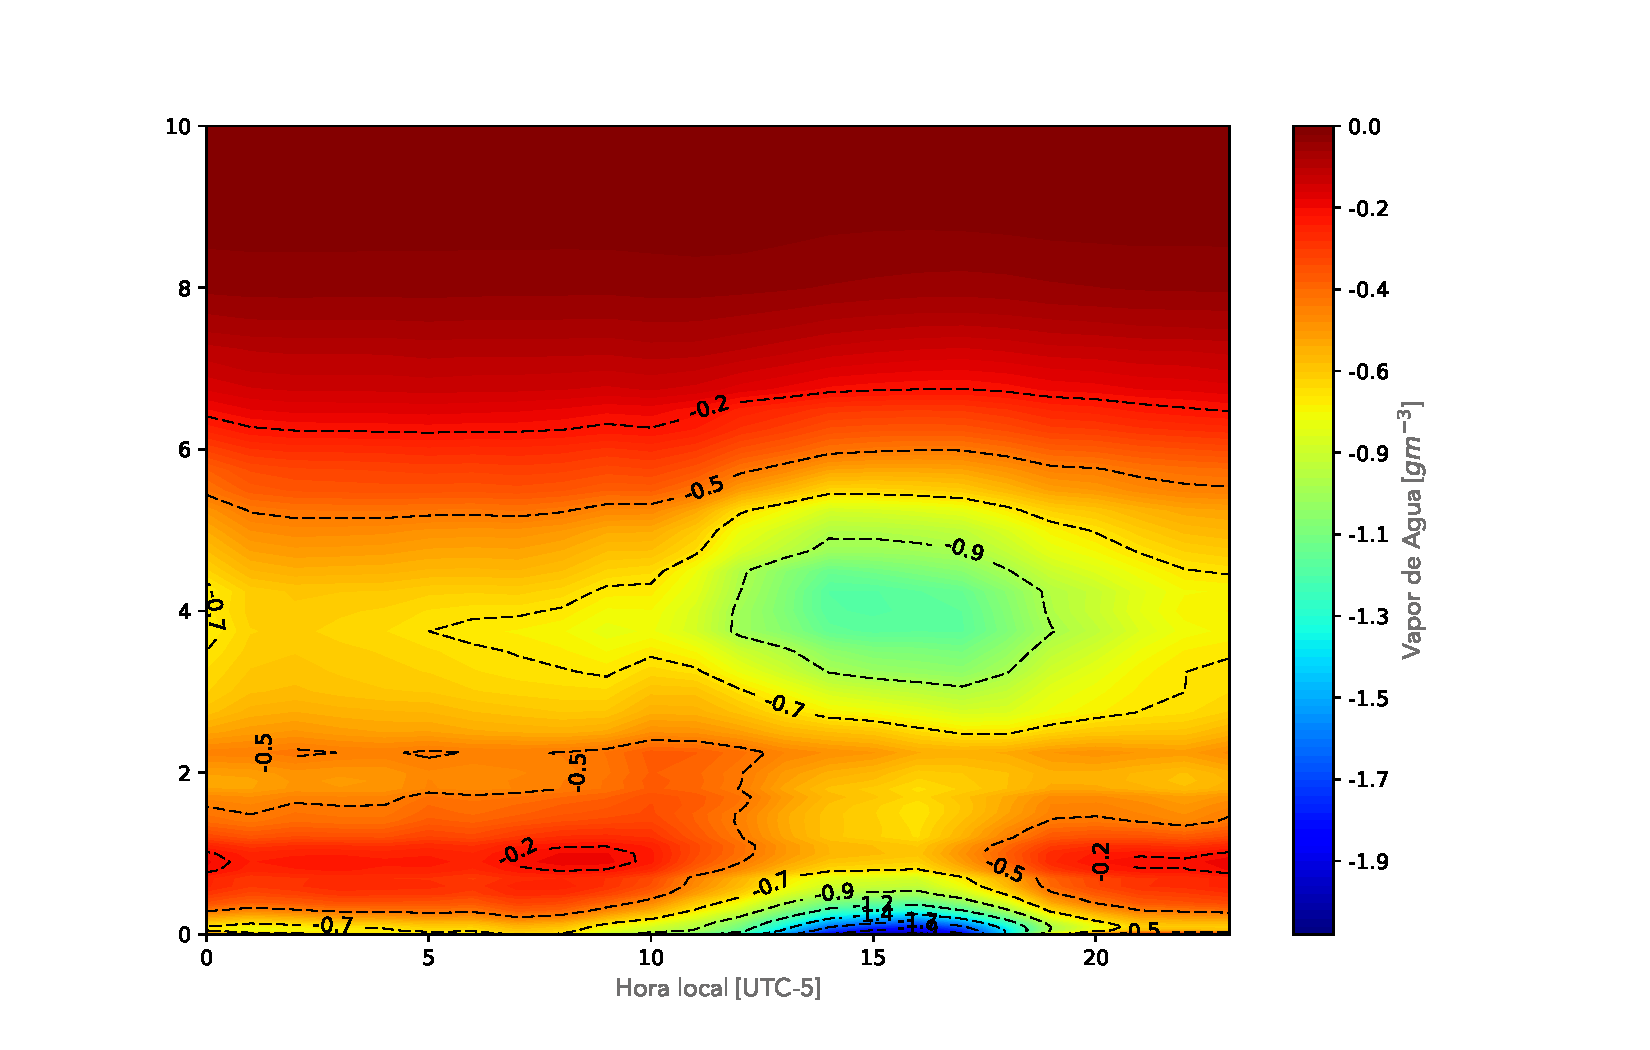
\includegraphics[width=1.2\linewidth]{Figuras/V_C_Matrix_resta.pdf}
\caption{Diurnal cycle difference of water vapour between days with absence or presence of precipitation events }
\label{fig:vapourDifference}
\end{figure}

The diurnal cycle  is not the only either the principal cycle in the variability of the water vapour and precipitation distribution, the annual cycle is another important component of the precipitation an water vapour variability due the radiative forcing, to analyze this cycle the Figure \ref{fig:VapDifference} shows the difference of the annual diurnal cycle of the integrated water vapour column between days with absence of precipitation and the days with presence of precipitation events. 

\begin{figure}[h!]
\centering
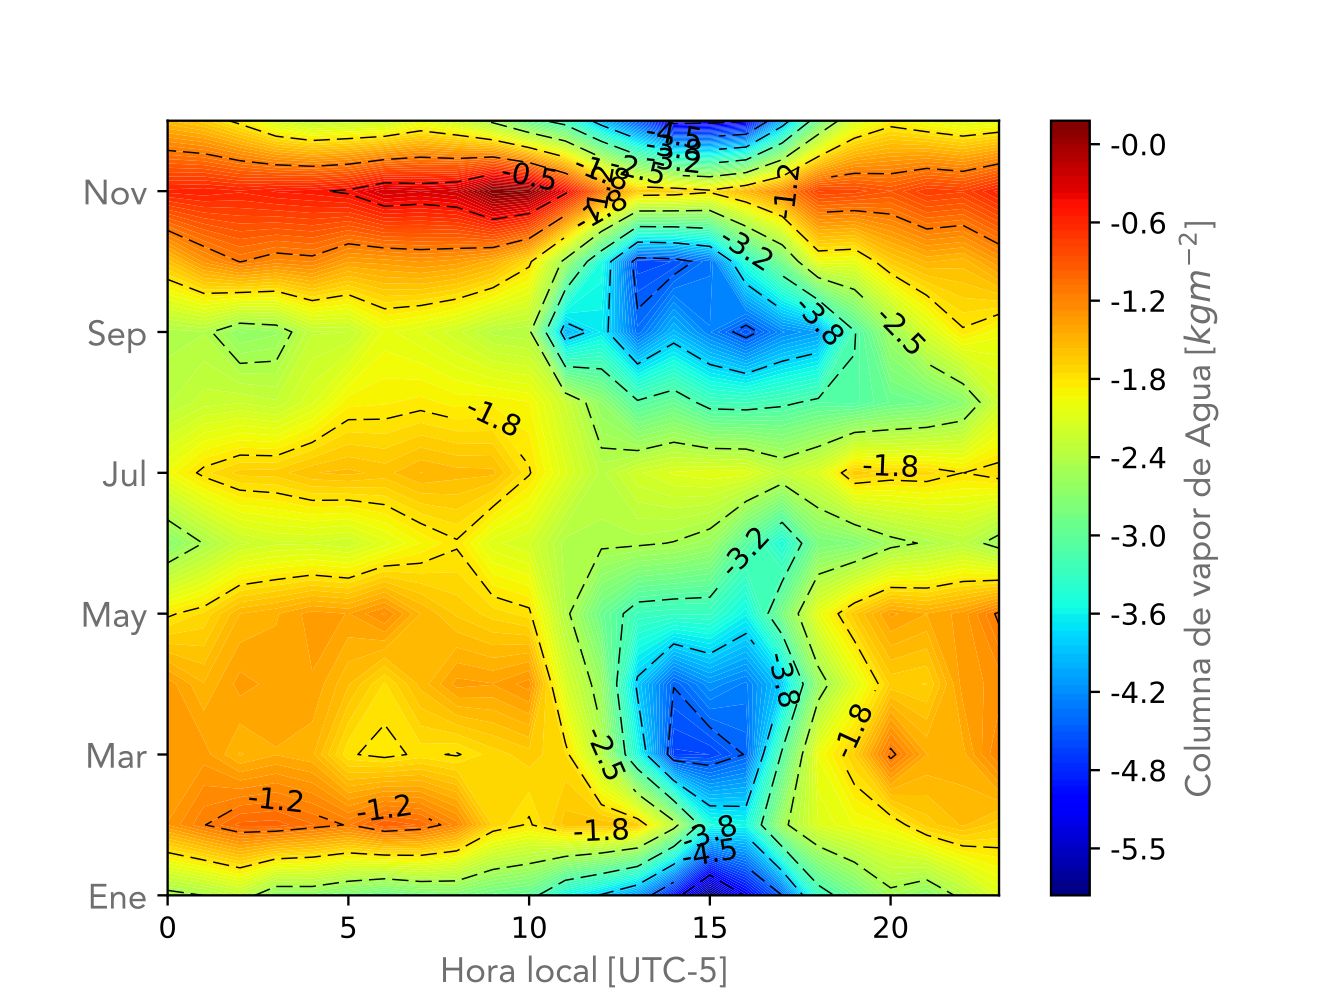
\includegraphics[width=1.0\linewidth]{Figuras/Vap_Resta_Matrix.png}
\caption{Annual diurnal cycle difference of integrated water vapour column between days with absence or presence of precipitation events }
\label{fig:VapDifference}
\end{figure}

The annual cycles modulates the quantity of precipitation and the availability of water vapour due to the passage of the Inter-Tropical Convergence Zone (ITCZ), that demarcates the two rainfall seasons in the colombia's andine zone 



\subsection{Stability indexes}

To analyze the atmospheric stability, i.e. thermodynamic profile, existing indexes that characterize, with an only value, the state of the thermodynamic profile of the atmosphere. The majority of the indexes were developed empirically with the purpose to measures the atmospheric instability for storm development, besides the indexes are commonly developed and tested in mid-latitude zones and flatlands, this increases the importance of evaluating the performance of this indexes in tropical zones with mountains and high altitudes and slopes. \textbf{(This is for try to define complex topography)}. Static stability indexes provide a simple representation of a complex aspect of the atmosphere and are widely used in operational forecasting. However, their applicability is limited, since most are specifically designed to measure deep instability \citep{henry2000static}.


\textbf{Define all indexes in the work, short with references, }

\subsubsection{Showalter index}
This is one of the first atmospheric stability index, made by \cite{showalter1953stability}. This index evaluates the instability between 850 and 500 hPa, with the buoyant energy at 500 hPa of an air parcel lifted from 850 hPa.


\begin{equation}
SI = T_{500} - T'_{\uparrow_{850}^{500} }
\label{eq:SI}
\end{equation}

where, $T_{500}$ is the ambient temperature at 500 hPa and $T'_{\uparrow_{850}^{500} }$ is the parcel temperature lifted adiabatically  from 850 to 500 hPa.\\
Is important emphasise, the Aburrá Valley bottom is at 1500 meters above mean sea level, near 850 hPa in pressure level, this implies that the parcel ascends is from the surface, different of the southwestern conditions use by Showalter in his study \citep{peppler1988review}.


\subsubsection{Lifted index}

Is a modification of Showalter index made by Galway \cite{galway1956lifted}, and is one of the most use instability index for storm forecasting \cite{peppler1988review}. Similarly, as the Showalter index, the lifted index evaluates the buoyant energy at 500 hPa of a parcel, but this parcel is adiabatically lifted from 50 hPa above the surface. 

\begin{equation}
LI = T_{500} - T'_{\uparrow_{sfc +50}^{500} }
\label{eq:LI}
\end{equation}

where, $T_{500}$ is the ambient temperature at 500 hPa and $T'_{\uparrow_{sfc +50}^{500} }$ is the parcel temperature lifted adiabatically  from 50 hPa above surface to 500 hPa. This is the principal difference with Showalter index in the calculation method.\\


\subsubsection{Convective Aviabable Pontential Energy, CAPE}
The before mentioned indexes are a function of the instability between two levels in the atmosphere. In addition, CAPE is the measurement of the parcel's buoyant energy above the level of free convection (LFC) and below of the level of neutral buoyancy (LNB), is the region where the parcel experiments positive buoyancy after the lifted condensation level (level of parcel's saturation). The amount of CAPE, calculate with the equation \ref{eq:CAPE}, represents the integral of buoyant energy between LFC and LNB, the humidity of the profile is considered in the use of virtual temperature. 
\begin{equation}
CAPE = \int_{LFC}^{LNB}g\tfrac{T'_v-T_v}{T_v}dz
\label{eq:CAPE}
\end{equation}

where  $T_v$ is the virtual temperature of the profile, $T'_v$ is the parcel's virtual temperature lifted from the surface, $g$ is the gravity attraction, $z$ is the height, $LFC$ is the level of free convection and $LNB$ is the level of neutral buoyancy.

\subsubsection{Convective INihibition Energy, CINE}
Is similarly calculate as CAPE, but represents the contrary favour to convection. This index represents the measures of energy in the stability region, i.e. (energy to no favours the lifting before LFC) is the region with negative buoyancy below LFC. In the particular case of Aburrá Valley, this index is an important key to understand the development of the atmospheric boundary layer and the convection 


\begin{equation}
CINE = \int_{SFC}^{LFC}g\tfrac{T'_v-T_v}{T_v}dz
\label{eq:CINE}
\end{equation}

where $SFC$ is the surface and the other terms are the same as the equation \ref{eq:CAPE}.


\textbf{Include the new graphs and the histograms, thinking to see be better the cycles, include hour precipitation separation}
Put comparision between AIRS, MWR and soundings
\begin{figure}[h!]
\centering
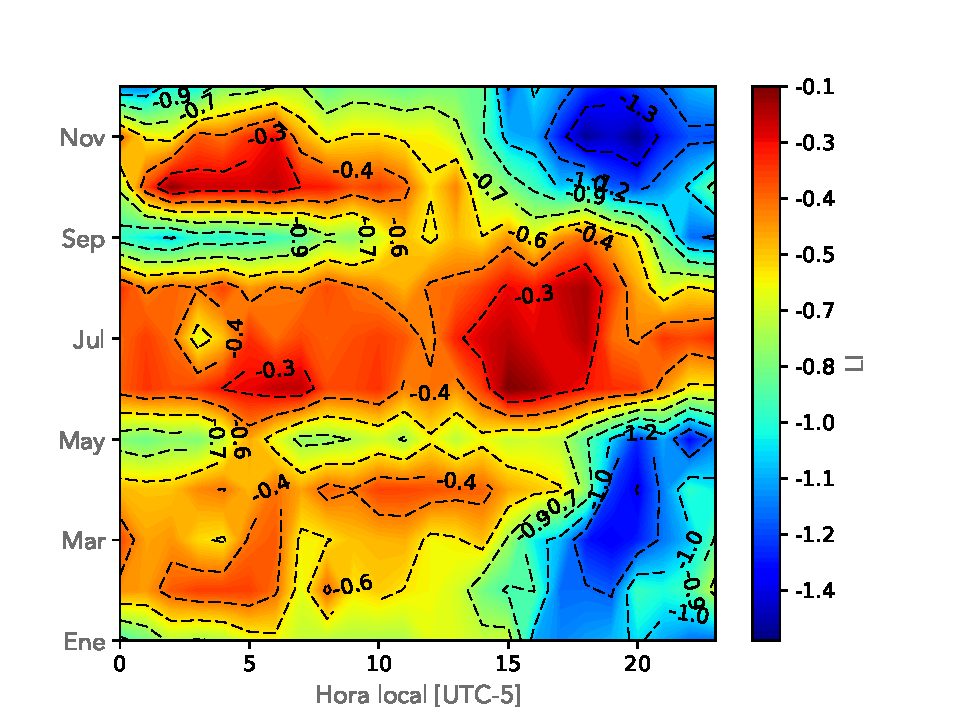
\includegraphics[width=1.0\linewidth]{Figuras/LI_Matrix_resta.pdf}
\caption{Diurnal cycle difference of CAPE between days with absence or presence of precipitation events }
\label{fig:LIdifference}
\end{figure}


\begin{figure}[h!]
\centering
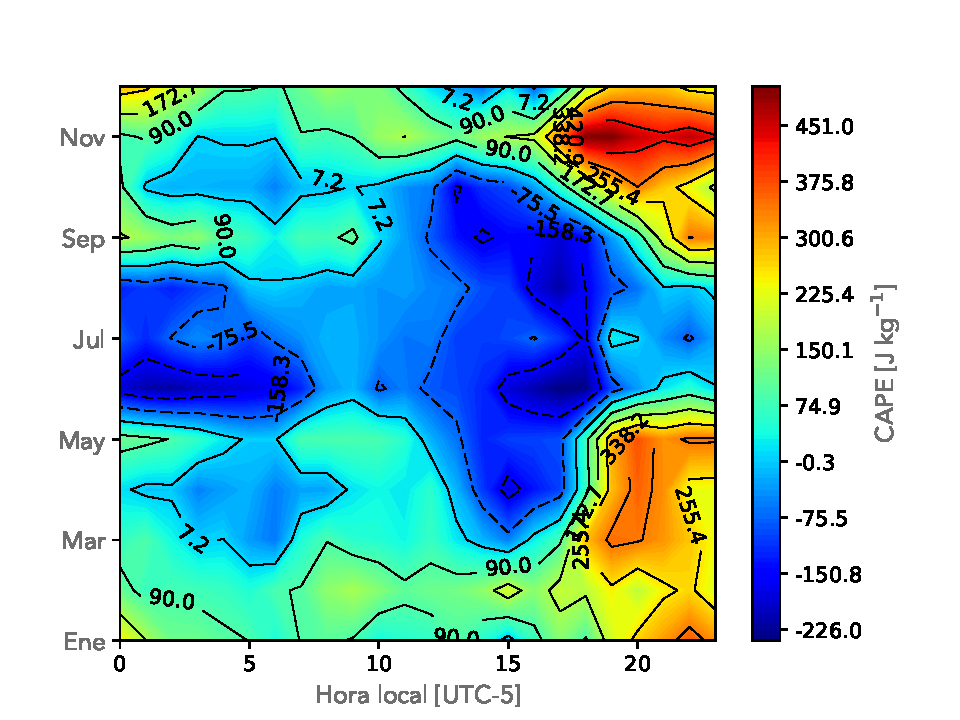
\includegraphics[width=1.0\linewidth]{Figuras/CAPE_Matrix_resta.pdf}
\caption{Diurnal cycle difference of CAPE between days with absence or presence of precipitation events }
\label{fig:CAPEdifference}
\end{figure}

The CAPE Shows the radiative forcing and also important is the more amount of energy available for the days with the absence of precipitation, this implicates that the days with precipitation events the potential convective energy is consumed in the precipitation


\begin{figure}[h!]
\centering
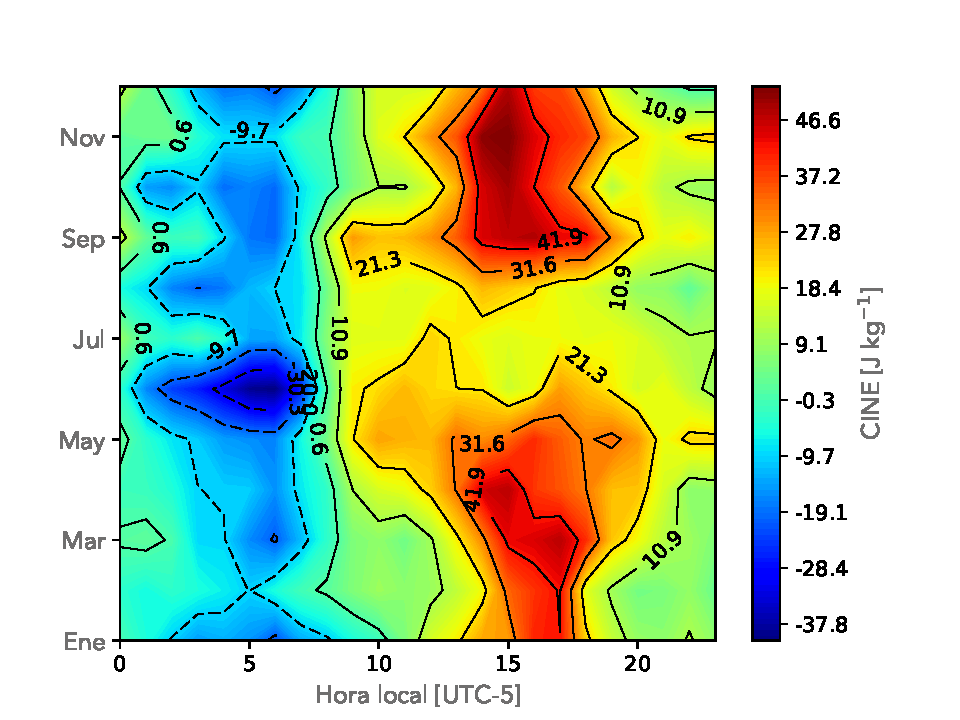
\includegraphics[width=1.0\linewidth]{Figuras/CINE_Matrix_resta.pdf}
\caption{Diurnal cycle difference of CINE between days with absence or presence of precipitation events }
\label{fig:CINEdifference}
\end{figure}


\begin{figure}[h!]
\centering
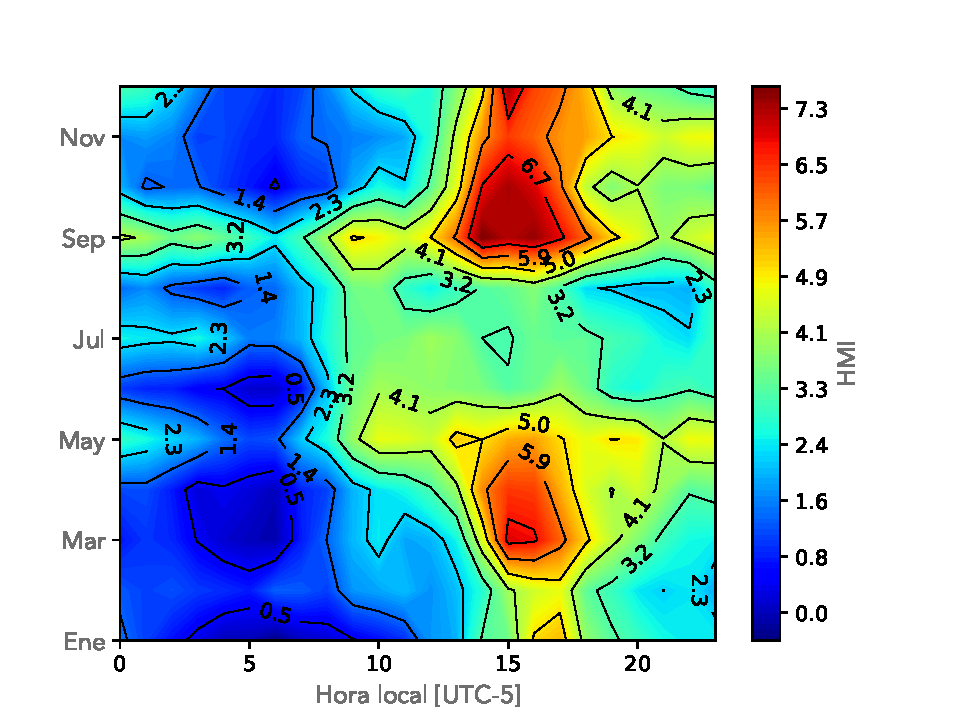
\includegraphics[width=1.0\linewidth]{Figuras/HMI_Matrix_resta.pdf}
\caption{Diurnal cycle difference of HMI between days with absence or presence of precipitation events }
\label{fig:HMIdifference}
\end{figure}

\section*{Data an methodology}
Water vapour sensing methods
\subsection*{AIRS}
Put a graphs an explanation about satellital monitoring, time scale and resolution
\subsection*{Microwave Radiometer}

\subsection*{Soundings}
Comparation with radiometer
\subsection*{WRF}
Comparation

\section*{Results}
Do the plot of histograms o all hours and months

\section*{Conclusions}


%%%%%%%%%%%%%%%%%%%%%%%%%%%%%%%%%%%%%%%%%%%%%%%%%%%%%%%%%%%%%%%%%%%%%
% FIGURES---PLACE AT END OF DOCUMENT
%%%%%%%%%%%%%%%%%%%%%%%%%%%%%%%%%%%%%%%%%%%%%%%%%%%%%%%%%%%%%%%%%%%%%
%\begin{figure}[h]
% \centerline{\includegraphics[width=19pc]{figure01.pdf}}
%  \caption{Enter the caption for your figure here.  Repeat as
%  necessary for each of your figures. Figure from \protect\cite{Knutti2008}.}\label{f1}
%\end{figure}
%


%%%%%%%%%%%%%%%%%%%%%%%%%%%%%%%%%%%%%%%%%%%%%%%%%%%%%%%%%%%%%%%%%%%%%
% TABLES---PLACE AT END OF DOCUMENT
%%%%%%%%%%%%%%%%%%%%%%%%%%%%%%%%%%%%%%%%%%%%%%%%%%%%%%%%%%%%%%%%%%%%%
%\begin{table}[h]
%\caption{This is a sample table caption and table layout.  
%Table from Lorenz (1963).}\label{t1}
%\begin{center}
%\begin{tabular}{ccccrrcrc}
%\topline
%$N$ & $X$ & $Y$ & $Z$\\
%\midline
% 0000 & 0000 & 0010 & 0000 \\
% 0005 & 0004 & 0012 & 0000 \\
% 0010 & 0009 & 0020 & 0000 \\
% 0015 & 0016 & 0036 & 0002 \\
% 0020 & 0030 & 0066 & 0007 \\
% 0025 & 0054 & 0115 & 0024 \\
%\botline
%\end{tabular}
%\end{center}
%\end{table}
%%

%%%%%%%%%%%%%%%%%%%%%%%%%%%%%%%%%%%%%%%%%%%%%%%%%%%%%%%%%%%%%%%%%%%%%
% ACKNOWLEDGMENTS
%%%%%%%%%%%%%%%%%%%%%%%%%%%%%%%%%%%%%%%%%%%%%%%%%%%%%%%%%%%%%%%%%%%%%
\acknowledgments
This work was supported by SIATA (Sistema de Alerta Temprana de Medellín y el Valle de Aburrá) funds provided by Area Metropolitana del Valle de Aburrá (AMVA), Municipio de Medellín, Grupo EPM, and ISAGEN under the Research and Technology Contract CD511, 2017, with Universidad EAFIT, institution that operates the early warning system. A special aknowledge to Mauricio Z..listar \citep{Hunter2007}.



%%%%%%%%%%%%%%%%%%%%%%%%%%%%%%%%%%%%%%%%%%%%%%%%%%%%%%%%%%%%%%%%%%%%%
% APPENDIXES
%%%%%%%%%%%%%%%%%%%%%%%%%%%%%%%%%%%%%%%%%%%%%%%%%%%%%%%%%%%%%%%%%%%%%

%% If only one appendix, use
%%\appendix%

%% If more than one appendix, use \appendix[<letter>], e.g.,
%  \appendix[A] 

% \appendixtitle{Title of Appendix}


% \subsection{Appendix section}

% The AMS template allows authors to format an unlimited number of
% appendixes. To format a single appendix, use the $\backslash$appendix
% command with no additional argument. Otherwise, add the appropriate
% one-letter argument to the $\backslash$appendix command (e.g.
% $\backslash$appendix[A], $\backslash$appendix[B],
% $\backslash$appendix[C], etc.) corresponding to the appropriate
% appendix. 


% The title of the appendix can be formatted using the
% $\backslash$appendixtitle{\tt\string{\string}} 
%  command. The $\backslash$subsection, $\backslash$subsubection,
% and $\backslash$paragraph commands are used to create sections within
% the appendix. (Note that the appendix title takes the place of $\backslash$section 
% in the appendix, so the first section should begin with $\backslash$subsection
% instead of $\backslash$section.)
%  Equations are automatically numbered appropriately for 
% each appendix. Here is an example of the first equation in appendix
% A, automatically labeled (\ref{eq:1}): 
% \begin{equation} \label{eq:1}
% x=\frac{2b\pm\sqrt{b^{2}-4ac}}{2c}.  
% \end{equation}

% For appendix figures and tables, special commands are needed to manually 
% change the numbering to ensure that each appendix figure or table is numbered 
% as part of the appendix and not as a continuation of the main paper. Use the command
% $\backslash$appendcaption\{\} instead of the usual $\backslash$caption\{\} to adjust the 
% numbering; for example, for Table A1, you would use the command \verb+\appendcaption{A1}+.
% In-text callouts for each appendix figure and table will need to be written as plain text;
% the usual $\backslash$ref\{\} command cannot be used.

% %%%%%%%%%%%%%%%%%%%%%%%%%%%%%%%%%%%
% %APPENDIX FIGURE AND TABLE EXAMPLES---PLACE AT END OF DOCUMENT
% %%%%%%%%%%%%%%%%%%%%%%%%%%%%%%%%%%%
% %
% %\begin{table}
% %\appendcaption{A1}{Here is the appendix table caption.}
% %\centering
% %\begin{tabular}{ccc}
% %a&b&c\\
% %d&e&f
% %\end{tabular}
% %\end{table}
% %
% %\begin{figure}
% %\centerline{(illustration here)}
% %\appendcaption{A1}{Here is the appendix figure caption.}
% %\end{figure}
% %


% \appendix[B]
% \appendixtitle{File Structure of the AMS \LaTeX\ Package}

% \subsection{AMS \LaTeX\ files}
% You will be provided with a tarred, zipped \LaTeX\ package containing 
% 17 files. These files are

% \begin{description}
% \item[Basic style file:] ametsoc.cls. 

% The file ametsoc.cls is the manuscript style file.  

% \begin{itemize}
% \item
% Using \verb+\documentclass{ametsoc}+ for your .tex document
% will 
% generate a PDF that follows all AMS guidelines for submission and peer
% review.  

% \item
% Using \verb+\documentclass[twocol]{ametsoc}+ for your .tex document
% can be used to generate a PDF that closely
% follows the layout of an AMS journal page, including single spacing and two
% columns.  This journal style PDF is only for the author's personal use, and
% any papers submitted in this style will not be accepted.  
% \end{itemize}
% Always use \verb+\documentclass{ametsoc}+ 
% when generating a PDF for submission to the AMS. 

% \item[Template:]
% template.tex, for the author to use when making his/her
% paper.
% The file provides a basic blank template with some
% section headings for authors to easily enter their manuscript.

% \item[Sample .tex and .pdf files:]
% The file amspaper.tex contains the \LaTeX\ code for the sample file.  
% The resulting PDF can be seen in amspaper.pdf (this file).


% \item[Sample article:] article formatted in draft and two-column mode.

% \begin{itemize}
% \item
% AMSSamp1.tex, AMSSamp1.pdf\\
% Formal paper done in draft mode and the resulting .pdf.

% \item
% AMSSamp2.tex, AMSSamp2.pdf \\
% The same paper using the \verb+[twocol]+ option and the resulting .pdf.

% \item
% FigOne.pdf, FigTwo.pdf, and figure01.pdf are sample figures.


% \end{itemize}

% \item[Bibliography Files:]

% ametsoc2014.bst, database2014.bib, and references.bib.  

% \begin{itemize}
% \item
% ametsoc2014.bst is the bibliography style file. 

% \item
% database2014.bib is an example of a bibliographic database file.

% \item
% references.bib should be altered with your own bibliography information.  
% \end{itemize}



% \item[Documention:] found in AMSDocs.pdf. Additional information
% found in
% readme.txt, which contains a list of the files and how they are used.

% \end{description}

% \subsection{Help for Authors}
% Questions and feedback concerning the use of the AMS \LaTeX\ files should be
% directed to latex@ametsoc.org. Additional information is available on the AMS
% \LaTeX\ Submission Info web page (\url{http://www2.ametsoc.org/ams/index.cfm/publications/authors/journal-and-bams-authors/author-resources/latex-author-info/}).



% \appendix[C]
% \appendixtitle{Building a PDF and Submitting Your 
% \LaTeX\ Manuscript Files to the AMS}

% \subsection{Building your own PDF}
% There are a variety of different methods and programs that will create a
% final PDF from your \LaTeX\ files. The easiest method is to download one of
% the freely available text editors/compilers such as TexWorks or TeXnicCenter.
% TexWorks is installed with the TeXLive distribution and provides both a text
% editor and the ability to compile your files into a PDF.

% \subsection{Submitting your files to the AMS for peer review}
% The AMS uses the Editorial Manager system for all author submissions for
% peer review. Editorial Manager uses the freely available \TeX\ Live 2011
% distribution. This system will automatically generate a PDF from your
% submitted \LaTeX\ files and figures.  

% You should not upload your own PDF into
% the system. If the system does not build the PDF from your files correctly,
% refer to the AMS \LaTeX\ FAQ page first for possible solutions. If your PDF
% still does not build correctly after trying the solutions on the FAQ page, email
% latex@ametsoc.org for help.

% \subsection{Other software}
% As mentioned above, there is a variety of software that can be used to edit
% .tex files and build a PDF.  The AMS does not support \LaTeX\/-related
% WYSIWYG software, such as Scientific Workplace, or WYSIWYM software, such as
% LyX.  \TeX\ Live (available online at \\ \url{http://www.tug.org/texlive/}) is
% recommended for users needing an up-to-date \LaTeX\ distribution with
% software that includes an editor and the ability to automatically generate a
% PDF.




%%%%%%%%%%%%%%%%%%%%%%%%%%%%%%%%%%%%%%%%%%%%%%%%%%%%%%%%%%%%%%%%%%%%%
% REFERENCES
%%%%%%%%%%%%%%%%%%%%%%%%%%%%%%%%%%%%%%%%%%%%%%%%%%%%%%%%%%%%%%%%%%%%%

\bibliographystyle{ametsoc2014}
\bibliography{Biblio}


%%%%%%%%%%%%%%%%%%%%%%%%%%%%%%%%%%%%%%%%%%%%%%%%%%%%%%%%%%%%%%%%%%%%%
% TABLES
%%%%%%%%%%%%%%%%%%%%%%%%%%%%%%%%%%%%%%%%%%%%%%%%%%%%%%%%%%%%%%%%%%%%%
% \begin{table}[h]
% \caption{This is a sample table caption and table layout.}\label{t1}
% \begin{center}
% \begin{tabular}{ccccrrcrc}
% \topline
% $N$ & $X$ & $Y$ & $Z$\\
% \midline
%  0000 & 0000 & 0010 & 0000 \\
%  0005 & 0004 & 0012 & 0000 \\
%  0010 & 0009 & 0020 & 0000 \\
%  0015 & 0016 & 0036 & 0002 \\
%  0020 & 0030 & 0066 & 0007 \\
%  0025 & 0054 & 0115 & 0024 \\
% \botline
% \end{tabular}
% \end{center}
% \end{table}
% %

% \begin{table}
% \appendcaption{A1}{Here is the appendix table caption.}
% \centering
% \begin{tabular}{ccc}
% \topline
% $1$ & $2$ & $3$ \\
% \midline
% a&b&c \\
% d&e&f \\
% \botline
% \end{tabular}
% \end{table}

%%%%%%%%%%%%%%%%%%%%%%%%%%%%%%%%%%%%%%%%%%%%%%%%%%%%%%%%%%%%%%%%%%%%%
% FIGURES
%%%%%%%%%%%%%%%%%%%%%%%%%%%%%%%%%%%%%%%%%%%%%%%%%%%%%%%%%%%%%%%%%%%%%



\end{document}
%%%%%%%%%%%%%%%%%%%%%%%%%%%%%%%%%%%%%%%%%%%%%%%%%%%%%%%%%%%%%%%%%%%%%
% END OF AMSPAPER.TEX
%%%%%%%%%%%%%%%%%%%%%%%%%%%%%%%%%%%%%%%%%%%%%%%%%%%%%%%%%%%%%%%%%%%%%